\documentclass{beamer}
\usepackage[utf8]{inputenc}
\usepackage[brazilian]{babel}

% Define as páginas de título das seções.
\newcommand{\sectiontitlepage}{
\begin{frame}
  \begin{center}
    \structure{\huge \insertsection}
  \end{center}
\end{frame}
}

\usetheme{Warsaw}
\setbeamercovered{transparent}
\setbeamertemplate{caption}[numbered]
\title{Introdução à Prototipagem de Sistemas Digitais em FPGA}
\author{Prof. Diego Cirilo}
\date{}
\institute[IFRN]{Instituto Federal de Educação, Ciência e Tecnologia do Rio Grande do Norte\\
                \textit{diego.cirilo@ifrn.edu.br}}

\begin{document}

\begin{frame}
\titlepage
\end{frame}

%\begin{frame}
%\frametitle{Sumário}
%\tableofcontents
%\end{frame}

\section{Conceitos}

\begin{frame}
  \frametitle{Scrum}
  \begin{itemize}[<+->]
    \item Desenvolvido nos anos 90 como forma de reduzir gargalos no processo de produção de software;
    \item Metodologia ágil, com foco na entrega do maior valor de negócio no menor tempo possível;
    \item As necessidades do negócio é que determinam as prioridades do desenvolvimento;
    \item Equipes auto organizadas para definir a melhor maneira de entregar as funcionalidades de maior prioridade;
    \item Revisão periódica da evolução do trabalho.
  \end{itemize}
\end{frame}

\begin{frame}{Conceitos}
  \begin{itemize}[<+->]
    \item Sprint: Período fixo onde objetivos serão definidos e resultados avaliados;
    \item Product Backlog: Conjunto de requerimentos e objetivos que existem para o projeto. Organizado em ordem de prioridade no quadro;
    \item Sprint Backlog (To do): Objetivos específicos que serão realizados no sprint seguinte, cada indivíduo escolhe o trabalho que fará.
  \end{itemize}
\end{frame}

\begin{frame}{Papéis (Roles)}
  \begin{itemize}[<+->]
    \item Product Owner: O dono do produto (cliente), quem define os requisitos básicos ou \textit{user stories} e prazos;
    \item Scrum Master: Mantém o funcionamento da equipe dentro das práticas do Scrum, resolvendo obstáculos e garantindo a colaboração entre os diversos papéis;
    \item Equipe: Responsável pela execução e divisão de tarefas (auto organizável).
  \end{itemize}
\end{frame}

\begin{frame}{Planejamento}
  \begin{itemize}[<+->]
    \item Reuniões de Sprint: É feita a avaliação do sprint anterior, verificando-se as tarefas que foram completadas ou não. Também onde o sprint backlog é criado com tarefas que a equipe se comprometa a entregar dentro do próximo período. Conta com a participação de todos;
    \item Reuniões diárias: Reunião de curta duração onde todos os membros apresentam a evolução e os obstáculos do dia anterior, além do planejamento para o dia atual;
  \end{itemize}
\end{frame}

\begin{frame}{Fluxo}
  \begin{figure}
    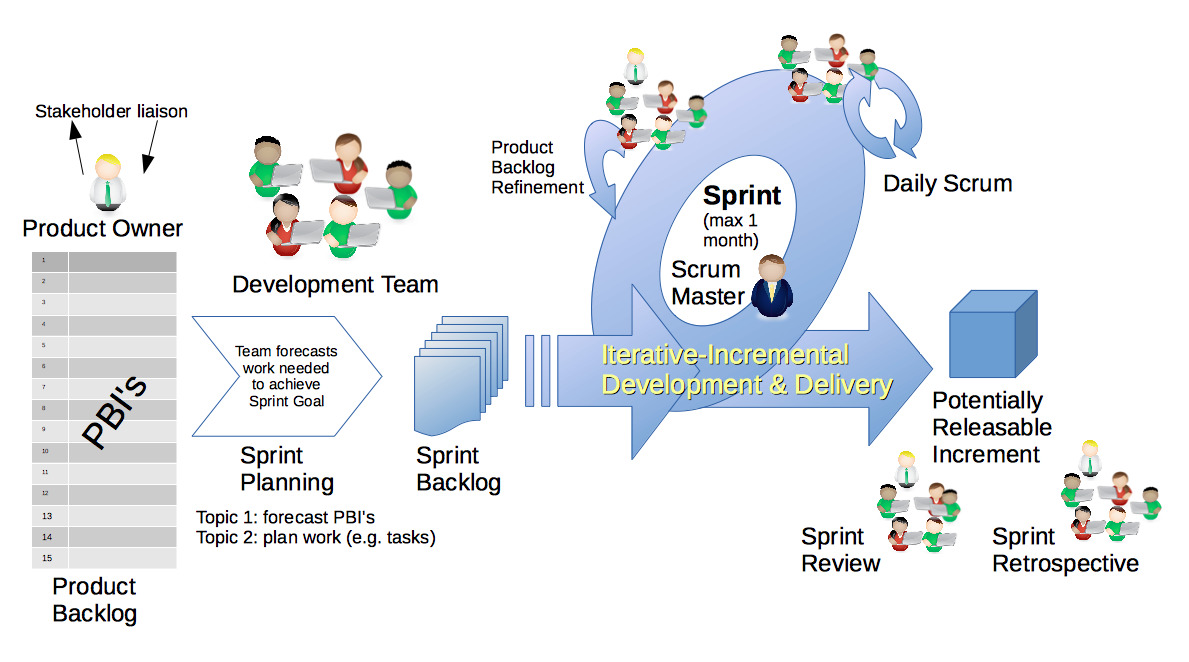
\includegraphics[width=10cm]{fig/scrum}
    \caption{Fluxo de trabalho}
    \label{fig:scrum}
  \end{figure}
\end{frame}

\begin{frame}{Scrum board}
  \begin{figure}
    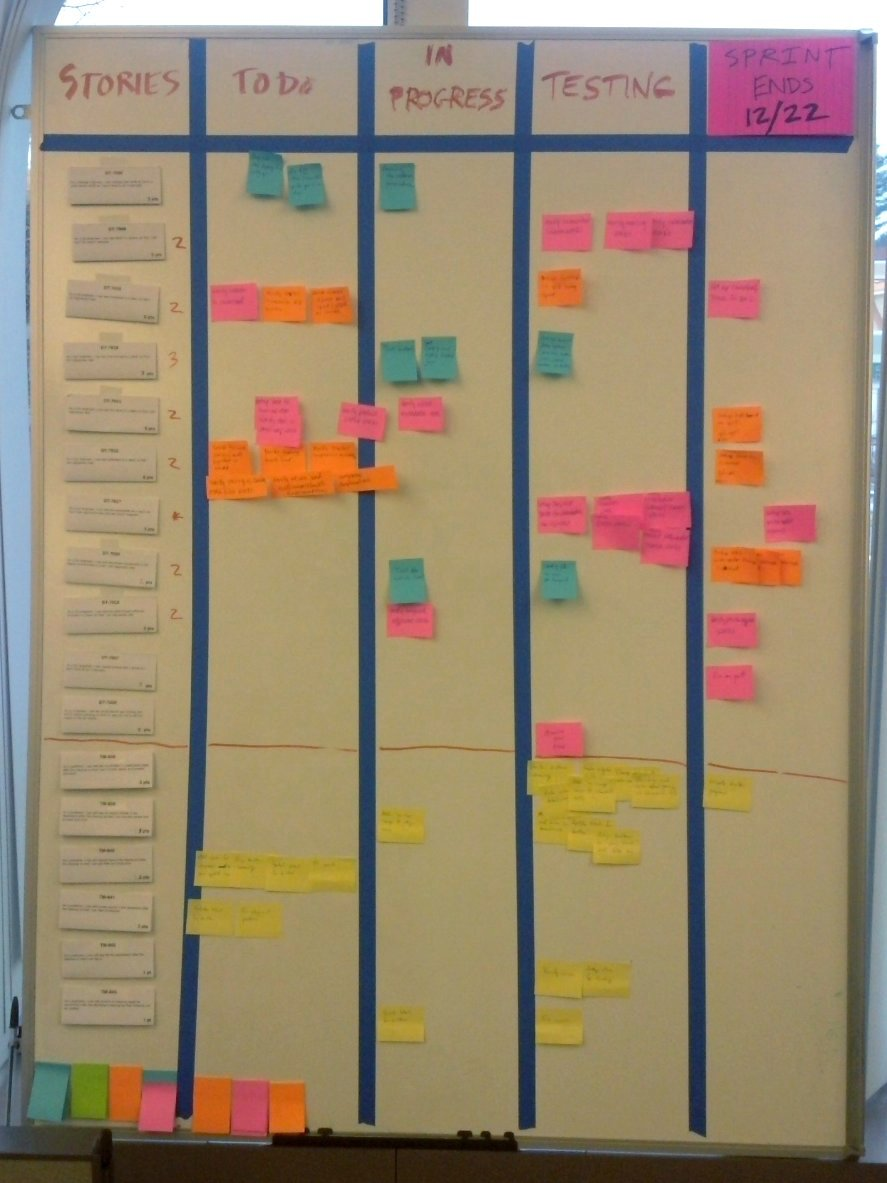
\includegraphics[width=5cm]{fig/board}
    \caption{Scrum board}
    \label{fig:board}
  \end{figure}
\end{frame}

\begin{frame}
  \frametitle{Dúvidas}
  \begin{center}
  \structure{\Huge ???}
  \end{center}
\end{frame}

\end{document}

